\section{Planificación, metodología y presupuesto}

En esta sección, se van a definir los componentes fundamentales en la gestión del proyecto. Estos permitirán definir claramente los objetivos, los recursos disponibles y cómo se utilizarán para alcanzar los resultados deseados dentro de un marco de tiempo y costos preestablecidos.

\subsection{Planificación temporal}

Se ha elaborado un calendario, marcando con colores los plazos (en días) de las distintas tareas y subtareas en las que se ha desglosado el proyecto.

\begin{figure}[H]
	\centering
	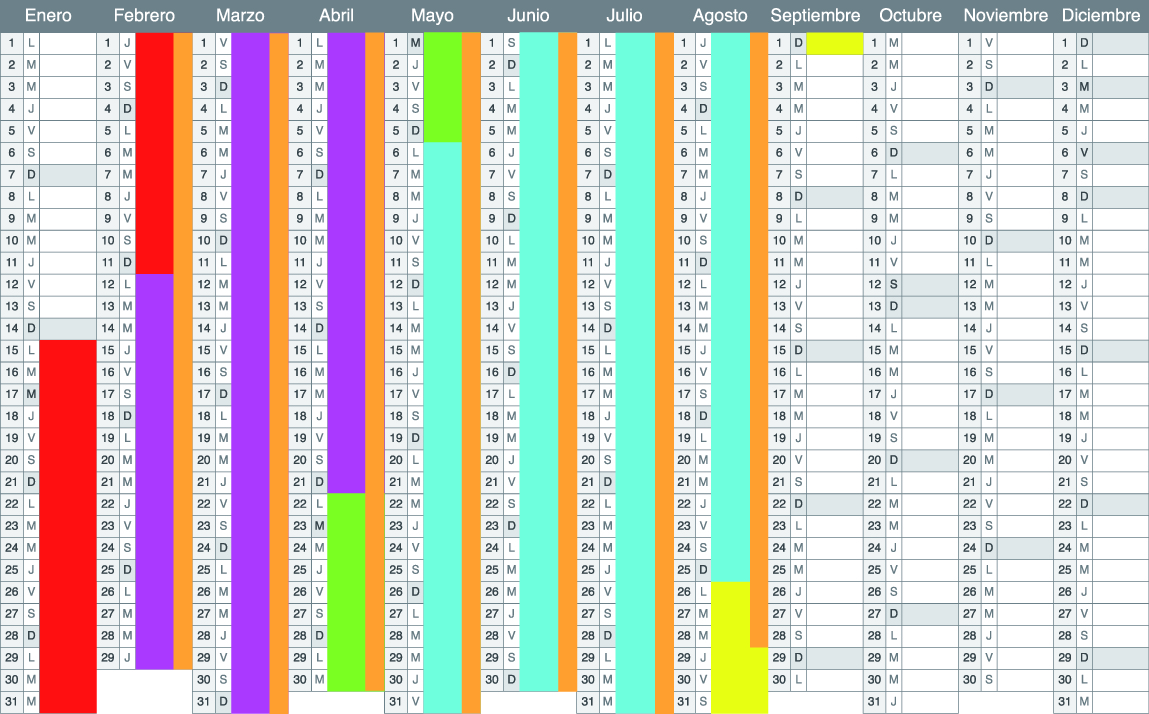
\includegraphics[width=1\textwidth]{imgs/tabla-planning1.jpg}
	\caption{Planificación temporal en el calendario}
	\label{fig:planning1}
\end{figure}

\begin{figure}[H]
	\centering
	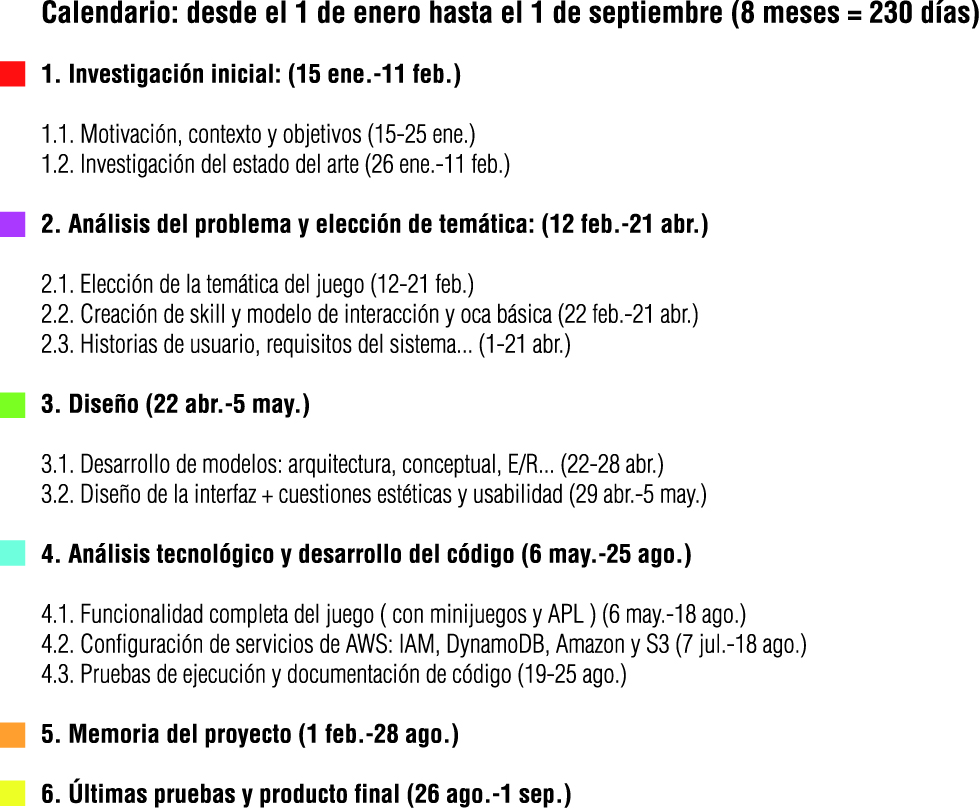
\includegraphics[width=1\textwidth]{imgs/tabla-planning2.jpg}
	\caption{Leyenda de la planificación temporal por (sub)tareas}
	\label{fig:planning2}
\end{figure}

\newpage
La planificación establece el marco temporal y los objetivos del proyecto dentro de las fechas límite para su entrega.

\begin{tabular}{|c|p{8cm}|c|c|c|}
	\hline
	\rowcolor{lightgray}
	\textbf{ID} & \textbf{Tarea} & \textbf{F. inicio} & \textbf{F. final} & \textbf{Duración (d.)} \\
	\hline
	\textbf{1.} & \textbf{Investigación inicial} & \textbf{15 ene.} & \textbf{11 feb.} & \textbf{28} \\
	\hline
	1.1. & Motivación, contexto y objetivos  & 15 ene. & 25 ene. & 11 \\
	\hline
	1.2. & Investigación del estado del arte & 26 ene. & 11 feb. & 17 \\
	\hline
	\textbf{2.} & \textbf{Análisis del problema y elección de temática} & \textbf{12 feb.} & \textbf{21 abr.} & \textbf{70} \\
	\hline
	2.1. & Elección de la temática del juego & 12 feb. & 21 feb. & 10 \\
	\hline
	2.2. & Creación de skill, modelo de interacción y oca básica & 22 feb. & 21 abr. & 59 \\
	\hline
	2.3. & Historias de usuario, requisitos del sistema... & 1 abr. & 21 abr. & 21 \\
	\hline
	\textbf{3.} & \textbf{Diseño} & \textbf{22 abr.} & \textbf{5 may.} & \textbf{14} \\
	\hline
	3.1. & Desarrollo de modelos: arquitectura, conceptual, E/R...  & 22 abr. & 28 abr. & 7 \\
	\hline
	3.2. & Diseño de la interfaz, cuestiones estéticas y usabilidad & 29 abr. & 5 may. & 7 \\
	\hline
	\textbf{4.} & \textbf{Análisis tecnológico y desarrollo de código} & \textbf{6 may.} & \textbf{25 ago.} & \textbf{112} \\
	\hline
	4.1. & Funcionalidad completa del juego (con minijuegos y APL) & 6 may. & 18 ago. & 106 \\
	\hline
	4.2. & Configuración de servicios de AWS: Amazon S3, IAM y DynamoDB  & 7 jul. & 18 ago. & 43 \\
	\hline
	4.3. & Pruebas de ejecución y documentación del código & 19 ago. & 25 ago. & 7 \\
	\hline
	\textbf{5.} & \textbf{Memoria del proyecto} & \textbf{1 feb.} & \textbf{28 ago.} & \textbf{210} \\
	\hline
	\textbf{6.} & \textbf{Últimas pruebas y producto final} & \textbf{26 ago.} & \textbf{1 sep.} & \textbf{7} \\
	\hline
	\rowcolor{lightgray}
	\textbf{} & \textbf{Conjunto total del proyecto} & \textbf{15 ene.} & \textbf{1 sep.} & \textbf{230} \\
	\hline
\end{tabular}


\subsection{Metodología}

La metodología describe las técnicas y procesos que se seguirán para desarrollar el proyecto, incluyendo las herramientas y tecnologías utilizadas, los roles y responsabilidades del equipo y los métodos de comunicación y gestión del proyecto. En este caso, se va a emplear la metodología de \textit{desarrollo ágil}.

El método de desarrollo ágil utiliza un enfoque iterativo y flexible, facilitando la adaptación a cambios y la entrega continua de valor al usuario. Esta metodología es especialmente efectiva en entornos donde las necesidades del usuario y el mercado pueden cambiar rápidamente, y donde la colaboración y la comunicación efectiva entre los miembros del equipo y con el cliente son fundamentales para el éxito del proyecto \parencite{metodologiaAgil}.

El desarrollo ágil para una aplicación se divide en varias etapas que se alinean con las prácticas y principios de dicha metodología. Estas fases incluyen:

\begin{enumerate}
    \item \textbf{Análisis del problema}: se centra en comprender las necesidades del usuario y los requisitos del sistema. En el contexto de una aplicación, implica la creación de historias de usuario y casos de uso, que son esenciales para definir las funcionalidades que la aplicación debe ofrecer.
    \item \textbf{Diseño}: se planifican las soluciones técnicas y se definen los detalles de diseño, como la arquitectura de la aplicación, el modelo E/R y el diseño de la interfaz de usuario. El diseño conceptual y los bocetos y mockups de esta fase preparan el camino para la implementación.
    \item \textbf{Desarrollo}: se trabaja para implementar las soluciones diseñadas. Esto incluye la codificación, integración de componentes y configuración del entorno de desarrollo.
    \item \textbf{Pruebas}: su realización permite corregir errores a tiempo. Esto asegura que la aplicación funcione como se espera y cumpla con los requisitos definidos en las etapas anteriores.
    \item \textbf{Despliegue}: una vez que la aplicación ha sido probada y se ha asegurado de que cumple con los requisitos y expectativas, se despliega para su uso.
    \item \textbf{Revisión y mejora continua}: tras el despliegue, se puede incluir la recopilación de comentarios de los usuarios, la identificación de áreas de mejora en el proceso de desarrollo y las implementaciones de cambios para mejorarla en iteraciones futuras.
\end{enumerate}


\subsection{Presupuesto}

El presupuesto es una herramienta clave para gestionar los recursos del proyecto, desde el asignamiento de recursos humanos hasta la adquisición de equipamiento y materiales necesarios. Permite estimar los costos asociados a cada entregable y recurso requerido, estableciendo un cronograma de gastos y asignando responsabilidades para el control de los mismos.

\subsubsection{Recursos humanos}
Incluye las personas involucradas en el proyecto, tanto en las etapas previas al desarrollo como durante el mismo.

\begin{table}[H]
    \centering
    \begin{tabular}{|c|c|}
    \hline
    \rowcolor{lightgray}
    \textbf{Descripción} & \textbf{Coste (€)}\\
    \hline
    Programador(a) & X \\
    \hline
    Psicólogo/a & X \\
    \hline
    \end{tabular}
    \caption{Presupuesto para recursos humanos}
    \label{tab:presupuesto-personal}
\end{table}

\subsubsection{Hardware}
Todos los dispositivos físicos y electrónicos necesarios para llevar a cabo la aplicación.

\begin{table}[H]
    \centering
    \begin{tabular}{|c|c|}
    \hline
    \rowcolor{lightgray}
    \textbf{Descripción} & \textbf{Coste (€)}\\
    \hline
    HP 15s Intel Core i5-1035G1/16GB/1TB/15.6" & 550-650 \\
    \hline
    Alexa Echo Show & 70 \\
    \hline
    \end{tabular}
    \caption{Presupuesto para hardware}
    \label{tab:presupuesto-hw}
\end{table}

\subsubsection{Software}
Los programas 

\begin{table}[H]
    \centering
    \begin{tabular}{|c|c|}
    \hline
    \rowcolor{lightgray}
    \textbf{Descripción} & \textbf{Coste (€)}\\
    \hline
    Visual Paradigm & 0 \\
    \hline
    Amazon Web Services (AWS) & X/? \\
    \hline
    Dynamo DB & X/? \\
    \hline
    Amazon S3 & X/? \\
    \hline
    TeXstudio & 0 \\
    \hline
    Visual Studio Code & 0 \\
    \hline
    Alexa Developer Console & 0 \\
    \hline
    \end{tabular}
    \caption{Presupuesto para software}
    \label{tab:presupuesto-sw}
\end{table}

\subsubsection{Resumen de presupuesto}
tfnjtrjrf

\begin{table}[H]
    \centering
    \begin{tabular}{|c|c|}
        \hline
        \rowcolor{lightgray}
        \textbf{Descripción} & \textbf{Coste (€)} \\
        \hline
        Recursos humanos & X \\
        \hline
        Hardware & X \\
        \hline
        Software & X \\
        \hline
    \end{tabular}
    \caption{Tabla general de presupuestos}
    \label{tab:presupuesto-total}
\end{table}
